\documentclass[tikz,border=3pt]{standalone}
\usepackage{fontspec}
\setmainfont{Helvetica}
\setsansfont{Helvetica}
\renewcommand{\familydefault}{\sfdefault}
\usepackage{xcolor}
\usetikzlibrary{calc}
\definecolor{tealSAC}{HTML}{0B6E75}
\definecolor{tealDark}{HTML}{084F55}
\definecolor{redCtrl}{HTML}{A94C43}
\definecolor{ink}{HTML}{253238}
\definecolor{muted}{HTML}{66757B}
\definecolor{gridline}{HTML}{D7DEE1}
\definecolor{amber}{HTML}{9A6A20}
\definecolor{c247D83}{HTML}{247D83}
\definecolor{c76ADB1}{HTML}{76ADB1}
\definecolor{c0F7077}{HTML}{0F7077}
\definecolor{c62A1A5}{HTML}{62A1A5}
\definecolor{c4D959A}{HTML}{4D959A}
\definecolor{cC9DEDF}{HTML}{C9DEDF}
\definecolor{cDDEAEA}{HTML}{DDEAEA}
\definecolor{c8BB9BC}{HTML}{8BB9BC}
\begin{document}
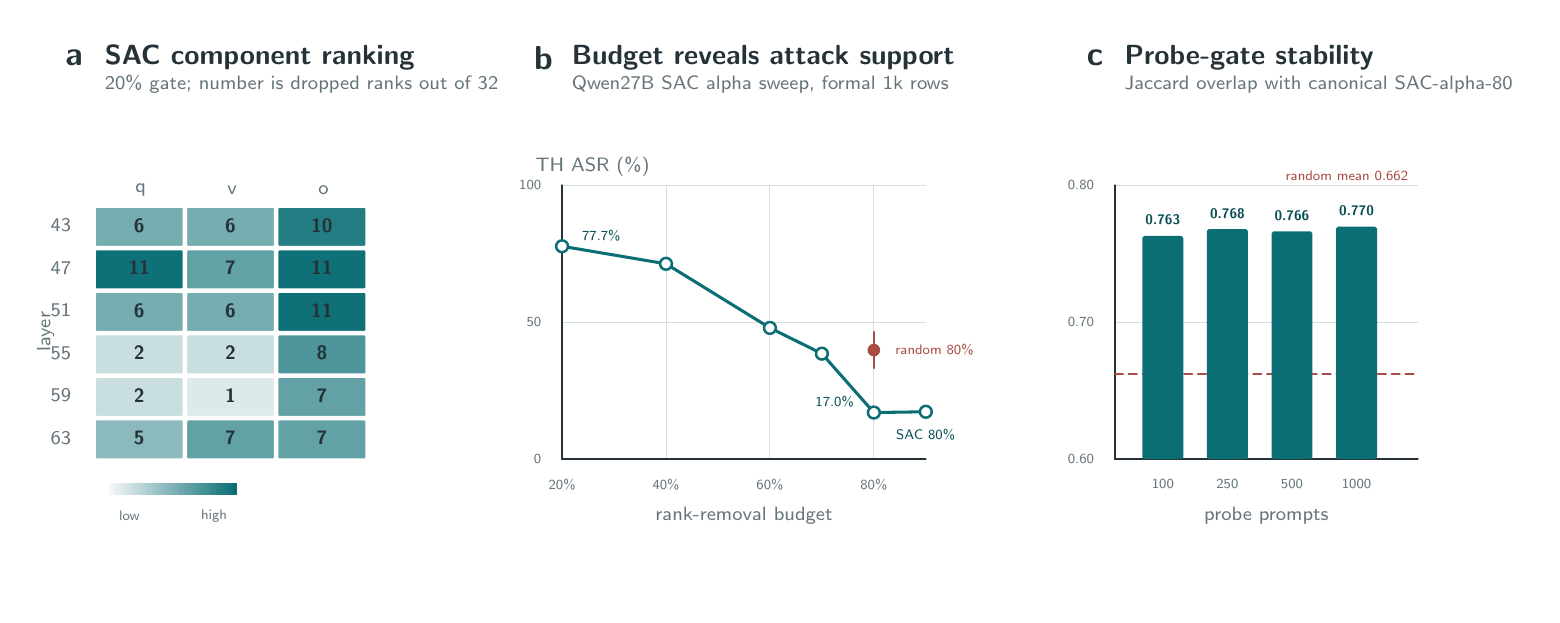
\begin{tikzpicture}[x=1cm,y=1cm,line cap=round,line join=round]
\fill[white] (0,0) rectangle (18.8,7.2);
\node[anchor=west,font=\bfseries\large,text=ink] at (0.05,6.82) {a};
\node[anchor=west,font=\bfseries,text=ink] at (0.55,6.82) {SAC component ranking};
\node[anchor=west,font=\scriptsize,text=muted] at (0.55,6.48) {20\% gate; number is dropped ranks out of 32};
\node[font=\scriptsize,text=muted] at (1.130,5.140) {q};
\node[font=\scriptsize,text=muted] at (2.290,5.140) {v};
\node[font=\scriptsize,text=muted] at (3.450,5.140) {o};
\node[anchor=east,font=\scriptsize,text=muted] at (0.370,4.690) {43};
\filldraw[fill=c76ADB1,draw=white,line width=0.5pt,rounded corners=0.4pt] (0.550,4.420) rectangle (1.670,4.920);
\node[font=\scriptsize\bfseries,text=ink] at (1.110,4.690) {6};
\filldraw[fill=c76ADB1,draw=white,line width=0.5pt,rounded corners=0.4pt] (1.710,4.420) rectangle (2.830,4.920);
\node[font=\scriptsize\bfseries,text=ink] at (2.270,4.690) {6};
\filldraw[fill=c247D83,draw=white,line width=0.5pt,rounded corners=0.4pt] (2.870,4.420) rectangle (3.990,4.920);
\node[font=\scriptsize\bfseries,text=ink] at (3.430,4.690) {10};
\node[anchor=east,font=\scriptsize,text=muted] at (0.370,4.150) {47};
\filldraw[fill=c0F7077,draw=white,line width=0.5pt,rounded corners=0.4pt] (0.550,3.880) rectangle (1.670,4.380);
\node[font=\scriptsize\bfseries,text=ink] at (1.110,4.150) {11};
\filldraw[fill=c62A1A5,draw=white,line width=0.5pt,rounded corners=0.4pt] (1.710,3.880) rectangle (2.830,4.380);
\node[font=\scriptsize\bfseries,text=ink] at (2.270,4.150) {7};
\filldraw[fill=c0F7077,draw=white,line width=0.5pt,rounded corners=0.4pt] (2.870,3.880) rectangle (3.990,4.380);
\node[font=\scriptsize\bfseries,text=ink] at (3.430,4.150) {11};
\node[anchor=east,font=\scriptsize,text=muted] at (0.370,3.610) {51};
\filldraw[fill=c76ADB1,draw=white,line width=0.5pt,rounded corners=0.4pt] (0.550,3.340) rectangle (1.670,3.840);
\node[font=\scriptsize\bfseries,text=ink] at (1.110,3.610) {6};
\filldraw[fill=c76ADB1,draw=white,line width=0.5pt,rounded corners=0.4pt] (1.710,3.340) rectangle (2.830,3.840);
\node[font=\scriptsize\bfseries,text=ink] at (2.270,3.610) {6};
\filldraw[fill=c0F7077,draw=white,line width=0.5pt,rounded corners=0.4pt] (2.870,3.340) rectangle (3.990,3.840);
\node[font=\scriptsize\bfseries,text=ink] at (3.430,3.610) {11};
\node[anchor=east,font=\scriptsize,text=muted] at (0.370,3.070) {55};
\filldraw[fill=cC9DEDF,draw=white,line width=0.5pt,rounded corners=0.4pt] (0.550,2.800) rectangle (1.670,3.300);
\node[font=\scriptsize\bfseries,text=ink] at (1.110,3.070) {2};
\filldraw[fill=cC9DEDF,draw=white,line width=0.5pt,rounded corners=0.4pt] (1.710,2.800) rectangle (2.830,3.300);
\node[font=\scriptsize\bfseries,text=ink] at (2.270,3.070) {2};
\filldraw[fill=c4D959A,draw=white,line width=0.5pt,rounded corners=0.4pt] (2.870,2.800) rectangle (3.990,3.300);
\node[font=\scriptsize\bfseries,text=ink] at (3.430,3.070) {8};
\node[anchor=east,font=\scriptsize,text=muted] at (0.370,2.530) {59};
\filldraw[fill=cC9DEDF,draw=white,line width=0.5pt,rounded corners=0.4pt] (0.550,2.260) rectangle (1.670,2.760);
\node[font=\scriptsize\bfseries,text=ink] at (1.110,2.530) {2};
\filldraw[fill=cDDEAEA,draw=white,line width=0.5pt,rounded corners=0.4pt] (1.710,2.260) rectangle (2.830,2.760);
\node[font=\scriptsize\bfseries,text=ink] at (2.270,2.530) {1};
\filldraw[fill=c62A1A5,draw=white,line width=0.5pt,rounded corners=0.4pt] (2.870,2.260) rectangle (3.990,2.760);
\node[font=\scriptsize\bfseries,text=ink] at (3.430,2.530) {7};
\node[anchor=east,font=\scriptsize,text=muted] at (0.370,1.990) {63};
\filldraw[fill=c8BB9BC,draw=white,line width=0.5pt,rounded corners=0.4pt] (0.550,1.720) rectangle (1.670,2.220);
\node[font=\scriptsize\bfseries,text=ink] at (1.110,1.990) {5};
\filldraw[fill=c62A1A5,draw=white,line width=0.5pt,rounded corners=0.4pt] (1.710,1.720) rectangle (2.830,2.220);
\node[font=\scriptsize\bfseries,text=ink] at (2.270,1.990) {7};
\filldraw[fill=c62A1A5,draw=white,line width=0.5pt,rounded corners=0.4pt] (2.870,1.720) rectangle (3.990,2.220);
\node[font=\scriptsize\bfseries,text=ink] at (3.430,1.990) {7};
\node[font=\scriptsize,text=muted,rotate=90] at (-0.080,3.340) {layer};
\definecolor{bar0}{HTML}{F2F6F6}
\fill[bar0] (0.730,1.270) rectangle (0.775,1.420);
\definecolor{bar1}{HTML}{EBF2F2}
\fill[bar1] (0.775,1.270) rectangle (0.820,1.420);
\definecolor{bar2}{HTML}{E5EEEF}
\fill[bar2] (0.820,1.270) rectangle (0.865,1.420);
\definecolor{bar3}{HTML}{DEEAEB}
\fill[bar3] (0.865,1.270) rectangle (0.910,1.420);
\definecolor{bar4}{HTML}{D8E6E7}
\fill[bar4] (0.910,1.270) rectangle (0.955,1.420);
\definecolor{bar5}{HTML}{D1E3E4}
\fill[bar5] (0.955,1.270) rectangle (1.000,1.420);
\definecolor{bar6}{HTML}{CADFE0}
\fill[bar6] (1.000,1.270) rectangle (1.045,1.420);
\definecolor{bar7}{HTML}{C4DBDC}
\fill[bar7] (1.045,1.270) rectangle (1.090,1.420);
\definecolor{bar8}{HTML}{BDD7D9}
\fill[bar8] (1.090,1.270) rectangle (1.135,1.420);
\definecolor{bar9}{HTML}{B7D3D5}
\fill[bar9] (1.135,1.270) rectangle (1.180,1.420);
\definecolor{bar10}{HTML}{B0CFD1}
\fill[bar10] (1.180,1.270) rectangle (1.225,1.420);
\definecolor{bar11}{HTML}{A9CBCD}
\fill[bar11] (1.225,1.270) rectangle (1.270,1.420);
\definecolor{bar12}{HTML}{A3C7CA}
\fill[bar12] (1.270,1.270) rectangle (1.315,1.420);
\definecolor{bar13}{HTML}{9CC3C6}
\fill[bar13] (1.315,1.270) rectangle (1.360,1.420);
\definecolor{bar14}{HTML}{96C0C2}
\fill[bar14] (1.360,1.270) rectangle (1.405,1.420);
\definecolor{bar15}{HTML}{8FBCBF}
\fill[bar15] (1.405,1.270) rectangle (1.450,1.420);
\definecolor{bar16}{HTML}{88B8BB}
\fill[bar16] (1.450,1.270) rectangle (1.495,1.420);
\definecolor{bar17}{HTML}{82B4B7}
\fill[bar17] (1.495,1.270) rectangle (1.540,1.420);
\definecolor{bar18}{HTML}{7BB0B4}
\fill[bar18] (1.540,1.270) rectangle (1.585,1.420);
\definecolor{bar19}{HTML}{75ACB0}
\fill[bar19] (1.585,1.270) rectangle (1.630,1.420);
\definecolor{bar20}{HTML}{6EA8AC}
\fill[bar20] (1.630,1.270) rectangle (1.675,1.420);
\definecolor{bar21}{HTML}{67A4A9}
\fill[bar21] (1.675,1.270) rectangle (1.720,1.420);
\definecolor{bar22}{HTML}{61A1A5}
\fill[bar22] (1.720,1.270) rectangle (1.765,1.420);
\definecolor{bar23}{HTML}{5A9DA1}
\fill[bar23] (1.765,1.270) rectangle (1.810,1.420);
\definecolor{bar24}{HTML}{54999E}
\fill[bar24] (1.810,1.270) rectangle (1.855,1.420);
\definecolor{bar25}{HTML}{4D959A}
\fill[bar25] (1.855,1.270) rectangle (1.900,1.420);
\definecolor{bar26}{HTML}{469196}
\fill[bar26] (1.900,1.270) rectangle (1.945,1.420);
\definecolor{bar27}{HTML}{408D92}
\fill[bar27] (1.945,1.270) rectangle (1.990,1.420);
\definecolor{bar28}{HTML}{39898F}
\fill[bar28] (1.990,1.270) rectangle (2.035,1.420);
\definecolor{bar29}{HTML}{33858B}
\fill[bar29] (2.035,1.270) rectangle (2.080,1.420);
\definecolor{bar30}{HTML}{2C8187}
\fill[bar30] (2.080,1.270) rectangle (2.125,1.420);
\definecolor{bar31}{HTML}{257E84}
\fill[bar31] (2.125,1.270) rectangle (2.170,1.420);
\definecolor{bar32}{HTML}{1F7A80}
\fill[bar32] (2.170,1.270) rectangle (2.215,1.420);
\definecolor{bar33}{HTML}{18767C}
\fill[bar33] (2.215,1.270) rectangle (2.260,1.420);
\definecolor{bar34}{HTML}{127279}
\fill[bar34] (2.260,1.270) rectangle (2.305,1.420);
\definecolor{bar35}{HTML}{0B6E75}
\fill[bar35] (2.305,1.270) rectangle (2.350,1.420);
\node[anchor=west,font=\tiny,text=muted] at (0.730,1.000) {low};
\node[anchor=east,font=\tiny,text=muted] at (2.350,1.000) {high};
\node[anchor=west,font=\bfseries\large,text=ink] at (6.00,6.82) {b};
\node[anchor=west,font=\bfseries,text=ink] at (6.48,6.82) {Budget reveals attack support};
\node[anchor=west,font=\scriptsize,text=muted] at (6.48,6.48) {Qwen27B SAC alpha sweep, formal 1k rows};
\draw[gridline,line width=0.35pt] (6.480,1.720) -- (6.480,5.200);
\node[font=\tiny,text=muted] at (6.480,1.400) {20\%};
\draw[gridline,line width=0.35pt] (7.800,1.720) -- (7.800,5.200);
\node[font=\tiny,text=muted] at (7.800,1.400) {40\%};
\draw[gridline,line width=0.35pt] (9.120,1.720) -- (9.120,5.200);
\node[font=\tiny,text=muted] at (9.120,1.400) {60\%};
\draw[gridline,line width=0.35pt] (10.440,1.720) -- (10.440,5.200);
\node[font=\tiny,text=muted] at (10.440,1.400) {80\%};
\draw[gridline,line width=0.35pt] (6.480,1.720) -- (11.100,1.720);
\node[anchor=east,font=\tiny,text=muted] at (6.340,1.720) {0};
\draw[gridline,line width=0.35pt] (6.480,3.460) -- (11.100,3.460);
\node[anchor=east,font=\tiny,text=muted] at (6.340,3.460) {50};
\draw[gridline,line width=0.35pt] (6.480,5.200) -- (11.100,5.200);
\node[anchor=east,font=\tiny,text=muted] at (6.340,5.200) {100};
\draw[ink,line width=0.55pt] (6.480,1.720) -- (11.100,1.720);
\draw[ink,line width=0.55pt] (6.480,1.720) -- (6.480,5.200);
\node[font=\scriptsize,text=muted] at (8.790,1.000) {rank-removal budget};
\node[anchor=west,font=\scriptsize,text=muted] at (6.020,5.440) {TH ASR (\%)};
\draw[tealSAC,line width=1.1pt] (6.480,4.424) -- (7.800,4.201);
\draw[tealSAC,line width=1.1pt] (7.800,4.201) -- (9.120,3.387);
\draw[tealSAC,line width=1.1pt] (9.120,3.387) -- (9.780,3.060);
\draw[tealSAC,line width=1.1pt] (9.780,3.060) -- (10.440,2.312);
\draw[tealSAC,line width=1.1pt] (10.440,2.312) -- (11.100,2.322);
\filldraw[fill=white,draw=tealSAC,line width=0.9pt] (6.480,4.424) circle (0.075);
\node[anchor=west,font=\tiny,text=tealDark] at (6.610,4.554) {77.7\%};
\filldraw[fill=white,draw=tealSAC,line width=0.9pt] (7.800,4.201) circle (0.075);
\filldraw[fill=white,draw=tealSAC,line width=0.9pt] (9.120,3.387) circle (0.075);
\filldraw[fill=white,draw=tealSAC,line width=0.9pt] (9.780,3.060) circle (0.075);
\filldraw[fill=white,draw=tealSAC,line width=0.9pt] (10.440,2.312) circle (0.075);
\node[anchor=east,font=\tiny,text=tealDark] at (10.310,2.452) {17.0\%};
\filldraw[fill=white,draw=tealSAC,line width=0.9pt] (11.100,2.322) circle (0.075);
\draw[redCtrl,line width=0.8pt] (10.440,2.876) -- (10.440,3.335);
\fill[redCtrl] (10.440,3.105) circle (0.08);
\node[anchor=west,font=\tiny,text=redCtrl] at (10.590,3.105) {random 80\%};
\node[anchor=west,font=\tiny,text=tealDark] at (10.600,2.032) {SAC 80\%};
\node[anchor=west,font=\bfseries\large,text=ink] at (13.02,6.82) {c};
\node[anchor=west,font=\bfseries,text=ink] at (13.50,6.82) {Probe-gate stability};
\node[anchor=west,font=\scriptsize,text=muted] at (13.50,6.48) {Jaccard overlap with canonical SAC-alpha-80};
\draw[gridline,line width=0.35pt] (13.500,1.720) -- (17.350,1.720);
\node[anchor=east,font=\tiny,text=muted] at (13.360,1.720) {0.60};
\draw[gridline,line width=0.35pt] (13.500,3.460) -- (17.350,3.460);
\node[anchor=east,font=\tiny,text=muted] at (13.360,3.460) {0.70};
\draw[gridline,line width=0.35pt] (13.500,5.200) -- (17.350,5.200);
\node[anchor=east,font=\tiny,text=muted] at (13.360,5.200) {0.80};
\draw[ink,line width=0.55pt] (13.500,1.720) -- (17.350,1.720);
\draw[ink,line width=0.55pt] (13.500,1.720) -- (13.500,5.200);
\draw[redCtrl,line width=0.6pt,densely dashed] (13.500,2.804) -- (17.350,2.804);
\node[anchor=east,font=\tiny,text=redCtrl] at (17.350,5.320) {random mean 0.662};
\fill[tealSAC,rounded corners=0.7pt] (13.850,1.720) rectangle (14.370,4.555);
\node[font=\tiny\bfseries,text=tealDark] at (14.110,4.755) {0.763};
\node[font=\tiny,text=muted] at (14.110,1.400) {100};
\fill[tealSAC,rounded corners=0.7pt] (14.670,1.720) rectangle (15.190,4.643);
\node[font=\tiny\bfseries,text=tealDark] at (14.930,4.843) {0.768};
\node[font=\tiny,text=muted] at (14.930,1.400) {250};
\fill[tealSAC,rounded corners=0.7pt] (15.490,1.720) rectangle (16.010,4.613);
\node[font=\tiny\bfseries,text=tealDark] at (15.750,4.813) {0.766};
\node[font=\tiny,text=muted] at (15.750,1.400) {500};
\fill[tealSAC,rounded corners=0.7pt] (16.310,1.720) rectangle (16.830,4.672);
\node[font=\tiny\bfseries,text=tealDark] at (16.570,4.872) {0.770};
\node[font=\tiny,text=muted] at (16.570,1.400) {1000};
\node[font=\scriptsize,text=muted] at (15.425,1.000) {probe prompts};
\end{tikzpicture}
\end{document}
